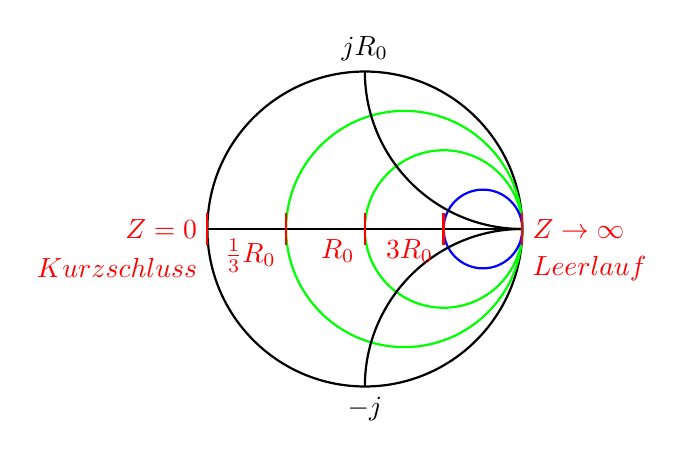
\begin{tikzpicture}[thick,dot/.style={fill=red,circle,minimum
size=1pt}]
	%einzigste Gerade
	\draw (-2,0) -- (2,0);
	%Kreise
	\draw (0,0) circle (2);
	\draw [green] (0.5,0) circle (1.5);
	\draw [green] (1,0) circle (1);
	\draw [blue] (1.5,0) circle (0.5);
	\draw (0,2) arc (180:270:2);
	\draw (0,-2) arc (180:90:2);
	%Rote bemerkungen
	\draw [red] (-2,0.2) -- (-2,-0.2);
	\draw [red] (-1,0.2) -- (-1,-0.2);
	\draw [red] (0,0.2) -- (0,-0.2);
	\draw [red] (1,0.2) -- (1,-0.2);
	\draw [red] (2,0.2) -- (2,-0.2);
	%Rote beschriftungen
	\node [red,anchor=east] at (-2,0) {$Z=0$};
	\node [red,anchor=east] at (-2,-0.5) {$Kurzschluss$};
	\node [red,anchor=north east] at (-1,0) {$\frac{1}{3}R_0$};
	\node [red,anchor=north east] at (0,0) {$R_0$};
	\node [red,anchor=north east] at (1,0) {$3R_0$};
	\node [red,anchor=west] at (2,0) {$Z\rightarrow\infty$};
	\node [red,anchor=west] at (2,-0.5) {$Leerlauf$};
	\node [anchor=south] at (0,2) {$jR_0$};
	\node [anchor=north] at (0,-2) {$-j$};
\end{tikzpicture}